\chapter{Implementation}

	In order to achieve the goals set in this project, two separate pieces of
	software and one piece of hardware were written. The software programs are
	two different implementations of a reference shader. The first of these was
	written in GLSL for traditional graphics hardware, and the second is written
	in an assembly language we designed for the Sphere Tracing processor. Both of
	these shaders are described in section \ref{implshader}.
	
	The hardware is comprised of a multi-core programmable parallel processing
	unit designed for the Sphere Tracing algorithm, detailed in section
	\ref{implproc}. In addition to these, a simple assembler program was written
	for the assembly language used for the GPU.
	
	\section{Shaders} \label{implshader}

		The shaders written uses the theory described in \ref{spheretracing}
		iterating over a ray in a main loop. The GLSL shader has more advanced
		optimizations added to it.

		\subsection{GLSL Based}
	
			The shader is made to run on conventional graphics hardware, it was
			created in the high-level shading language GLSL (short for OpenGL
			Shading Language). It runs the program for each pixel the shader is
			rendered on, using the screen-coordinates as input.
			
			Before the loop is run Orthogonal Culling is executed, reducing the
			number of objects in the distance field. Beyond this, objects can
			also be enclosed in Bounding Spheres.
			
			After a hit is detected different things happen depending on the material
			assigned to the object. If the object is reflective, then the normal of the
			surface hit is calculated and used to reflect the ray. If the object is
			colored the pixel will simply be set according to the object. Color can
			also be calculated from object or ray coordinates. Coloring the pixel
			depending on where the object is or where it was hit.

		\subsection{Orthogonal Culling}

			A bottleneck of Sphere Tracing is that the distance to a lot of objects
			has to be calculated once for every march step. Performance can be
			increased by reduceing the number of objects that the distance has to be
			calculated to, without reducing the actual number of objects in the
			scene. To do this the GPU needs to calculate which object a ray might hit
			by checking its field of view. This information is traditionally
			calculated on the CPU and then passed to the GPU (Frustum culling). Even
			frustum culling might not be enough. Each ray should only care about the
			objects that it might hit, not all objects in the field of view.

			Orthogonal Culling works by going through all the objects in the scene
			and calculate what rays might hit what object. Orthogonal projection is
			used to tell whether a object is in front of the ray or not. By
			projecting the center of the sphere onto the directional line of the ray,
			its the line's closest point to the object is known. Then the distance
			between the line and the sphere can be calculated using the radius, if
			the distance is less than zero the sphere will be hit by the ray. If the
			distance is larger than zero the ray can't possibly hit that sphere. This
			way the number of objects that the distance has to be calculated to is
			decreased.

		\subsection{Bounding Spheres}
			
			In order to decrease the number of distance calculations that has to be
			performed in each march step, objects can be grouped together in larger
			enclosing bounding spheres. When the distance field is evaluated only the
			bounding sphere will be considered and none of the objects enclosed by
			it. If the bounding sphere is hit by the ray, it will be removed and all
			the contained objects will be introduced to the distance field.
			
			A Bounding Sphere is defined by it's location, radius and enclosed
			objects. The location is calculated by adding the position-vectors
			of objects and scaling the result with the inverse of the number of
			objects. The radius is the distance to the object that is the
			furthest from the Bounding Sphere's position added to that objects
			sphere of influence (how far it reaches from it's origin). This
			way there is no risk of objects being partially rendered.


		\subsection{Assembler Based}

			In this shader no optimizations were implemented. Initially a single
			thread is created, it is used to create new threads and push them to the
			queue. One thread will be created for each pixel on the screen, and also
			an id will be given to each thread. This id corresponds to a pixel to the
			screen.  An example: If the resolution of the display is 2x2 4 threads
			will be created and given id's ranging from 4 to 1. Once all threads have
			been instantiated the initial thread will be terminated.

			When a new thread is created the screen coordinates is calculated 
			from the thread id, this is essential for calculating the ray 
			direction. As with the software shader, camera position and a point 
			to orient the camera against is predefined. 

			After screen coordinates are calculated a ray direction vector is
			calculated, after this all initial setup calculations are done. The
			Sphere Tracing loop is a straight-forward implementation of the 
			algorithm. If a hit is detected a flat color will be assigned to 
			the corresponding pixel.

	\section{Processor Unit} \label{implproc}

		The properties of the ray marching algorithm as described in chapter
		\ref{spheretracing} led to the decision of designing a GPU architecture
		that does not utilize multi-ALU SIMD with lockstepping to the same
		extent as that of traditional graphics processors. Instead, a solution 
		with slightly simpler independent cores was decided upon. This is 
		similar to reasoning employed by \cite{Woop2005} for a Ray Tracing 
		hardware design.

		The hardware described in this section was written in \clash. \clash is
		based on the functional programming language Haskell and is therefore a
		functional hardware description language, or FHDL.

		\subsection{Architecture}

			The GPU is designed to be able to handle a form of threading
			natively, where all computations are performed by a thread running
			on a hardware core. A thread in this context is very light-weight:
			only an instruction pointer along with some mutable registers are
			stored.

			All threads that are not running are sent to a storage manager that
			communicates with all cores, and threads are then dispatched to
			cores as the cores become available for execution. The cores are
			also able to spawn new threads by sending their data to the storage
			manager, or terminate their current threads either by simply
			dropping them or by sending them to the frame buffer, where some of
			the registers will be used to determine the color of some pixel on
			the screen.

			The storage in the storage manager on the XQBGPPPU is implemented
			as a double-ended queue. This makes it possible for threads to have
			some coarse-grained control over execution priority, which is
			needed in order for many types of programs to be able to run with a
			bunded number of threads at any given time. During execution, the
			storage manager selects one core that is ready to send a thread, if
			any core is ready to do so, and adds its thread to the storage. If
			any core is ready to receive a thread, one is taken from the 
			storage and sent to that core. If more than one core is ready, one
			is chosen arbitrarily.

			Each core consists of instruction and data memories, some control 
			logic for execution order and a DFU. The data and instruction 
			memories are immutable and mirrored across all cores in their 
			entirety. The control logic is responsible for feeding the DFU with
			instructions and data, as well as updating the thread registers 
			when a new thread is attached, sending thread registers to the 
			storage manager when new threads are spawned and and 
			requesting a new thread whenever the previously executing one 
			terminates.
			
			The DFU contains a stack which all arithmetic instructions operate
			on, as well as an ALU for carrying out calculations. It also keeps
			track of all the thread registers and updates them when such
			instructions are issued. The DFU contains very little extra control
			logic and is only able to receive and execute instructions, it does
			not keep track of any instruction pointers or when threads are
			attached or dropped, this is instead handled by the core control
			logic.

		\subsection{Instruction Set}

			A representation for distance functions was also designed. It is
			implemented as a reverse polish notation inspired stack based 
			instruction set.

			There are a total of four instruction types with different
			instruction encodings, their layout in memory is shown in figure
			\ref{encodingfig}, and the type of instructions are:

			\begin{description}
				\item[C-type] instructions are for control flow, that is, 
					instructions that affect the global queue or frame buffer or
					terminate the current thread. C-type instructions can be 
					conditionally executed, based on the condition encoded in
					the two highest bits in the opcode. 

				\item[D-type] instructions, which encode arithmetic- and vector
					instructions on the stack. These operate only on the
					internal stack in the core and not on any of the other
					registers. They can take up to six arguments and return up
					to three return values. D-type instructions can be split up
					in chunks using the \texttt{next} instruction, where the
					last computed result will be accumulated using the minimum
					automatically by the core. This is useful for encoding
					distance functions.

				\item[V-type] instructions deal with memory accesses. The
					\texttt{p} bit encodes whether this access is for pack
					(mutable) or read-only memory.

				\item[R-type] instructions load wide immediate values into the
					DFU. They are currently only used for assigning distance
					function IDs.
			\end{description}

		\subsection{Execution Model}

			The processor contains a global storage structure that is shared
			among all cores by a storage manager. All threads that are 
			ready for execution are held in this storage until a core is ready 
			to start executing them.

			\begin{figure}[H]
				\centering
				\caption{ XQBGPPPU Data flow diagram }
					\includegraphics[width=0.75\linewidth]{figure/dots/GPU-schematic} 
				\vspace{-4pt}
			\end{figure}
	
			Each shader thread has 16 mutable registers that are automatically
			loaded into the core when execution starts. These registers are
			saved when execution pauses and copied whenever a thread spawns a 
			new child. The instruction \texttt{setval} can be used to change 
			the value of a register, and the instruction \texttt{pack} reads 
			the value of a register.

			All calculations are performed with intermediate values stored on a
			stack, with the ability to move any values between the stack and
			any of the registers using the \texttt{setval} and \texttt{pack}
			instructions.

			There are three main instructions for control flow: \texttt{pushq},
			\texttt{pushf}, and \texttt{drop}. Threads can spawn new threads at
			any time using the instruction \texttt{pushq}: this will cause the
			core to make a copy of all of the registers and push it onto the
			global queue, where another (or the same) core may later access
			them and start executing from the instruction pointer register
			(\texttt{r0}).

			Threads can also terminate execution in two ways. Executing the
			instruction \texttt{drop} will terminate the thread and discard all
			registers. Executing \texttt{pushf} will terminate the thread and
			discard all values except the pixel pointer (\texttt{r1}) and color
			register (\texttt{r2}), which will be sent to the frame buffer in
			order to be displayed on the screen.

			This set of instructions for control flow might initially seem to
			be neither useful nor easy to implement but they are powerful
			enough to implement for all branching that is needed in our ray
			marchers efficiently while being restrictive enough to make
			instruction memory accesses very predictable.

			In addition to this, each core can accelerate finding the minimum 
			distance for a set of distance functions using a built-in 
			accumulator, together with the instructions \texttt{next} and 
			\texttt{accum}. Because of this, distance functions can be written
			without any regard for how the shader that called them works, and
			this very common operation is automated, reducing the size of each
			distance function slightly.

		\subsection{Square Roots}

			Calculating distances is an integral part of the algorithm, so a
			good square root implementation was considered important for
			achieving good performance. Several different approaches for this
			were considered.

			Firstly, using an iterative method like Goldschmidt's or the
			babylonian method was considered. These require an initial starting
			value, which is usually generated using a look-up table. We tested
			a different and very fast method for generating an initial rough
			guess of the square root of any number without the need for a
			look-up table. A 16-bit version of this circuit is shown in figure
			\ref{orsqrt}, and an improved but slightly more expensive version
			is showed in figure \ref{orsqrt2}. The basic working principle is
			based on the fact that the square root of a number has roughly half
			as many digits as the original number. In the version with slightly
			improved accuracy the placement of the extra wires is based on the
			bit pattern of $\sqrt{2}$.

			\begin{figure}
				\centering
				\caption{A simple square root approximator}
				\label{orsqrt}
				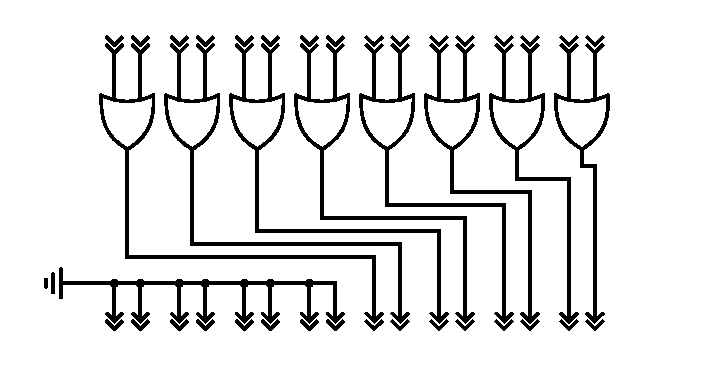
\includegraphics[width=0.75\linewidth]{figure/pdf/simpleOr.pdf} 
			\end{figure}

			\begin{figure}
				\centering
				\caption{Simple square root approximator with minor improvement.
					More layers of or-gates can be added with increased shifts 
					for slight increases in accuracy. }
				\label{orsqrt2}
				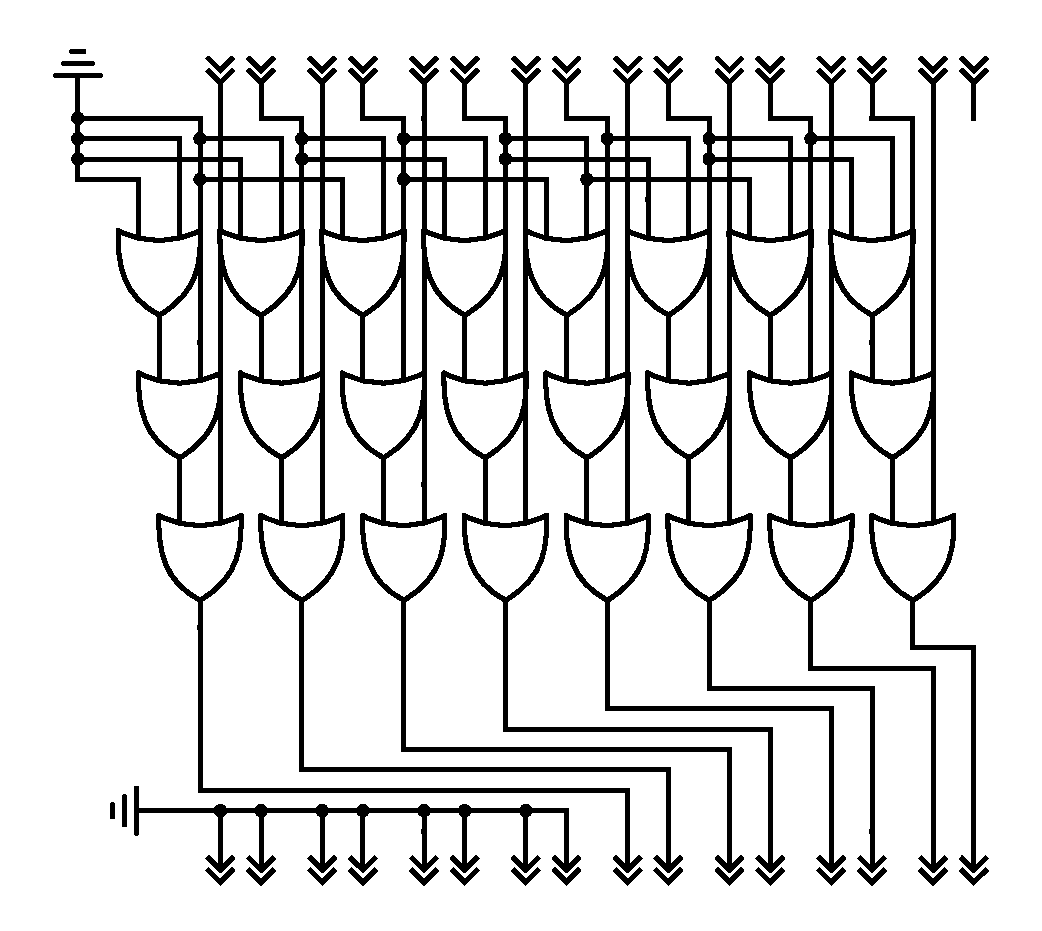
\includegraphics[width=0.75\linewidth]{figure/pdf/sqrt3Or.pdf} 
			\end{figure}

			In order to improve upon this method, both in terms of accuracy and
			stability, another design was considered in which the input was
			both rounded up and down to values where the simple square root
			approximator was very accurate and the result was then linearly
			interpolated between these roots. This linear interpolation
			requires only a multiplication and a couple of additions, but
			choosing upper and lower seed values is a more complex problem.
			Choosing the two geometrically closest powers of two was tested
			because the or-gate square root circuit is very accurate for powers
			of two, but this is not the only possible choice, as there are many 
			points for which the simple square root approximator is very 
			accurate. We did not look further into choosing different upper and
			lower bounds for the lerp-approximator.

			\begin{figure}
				\centering
				\caption{ Simple square root approximator used together with
					linear interpolation. This version includes an extra layer
					of or-gates with a shift of 4 and is more accurate for
					powers of 2. Note that the gates in this diagram seem to be
					ordered in two extra layers. This is, however, only a
					visual artifact in this image. Adding more layers with
					shifts of 6, 10, 14, 26 etc increases accuracy further,
					although returns are diminishing quickly.}
				\label{orsqrt3}
				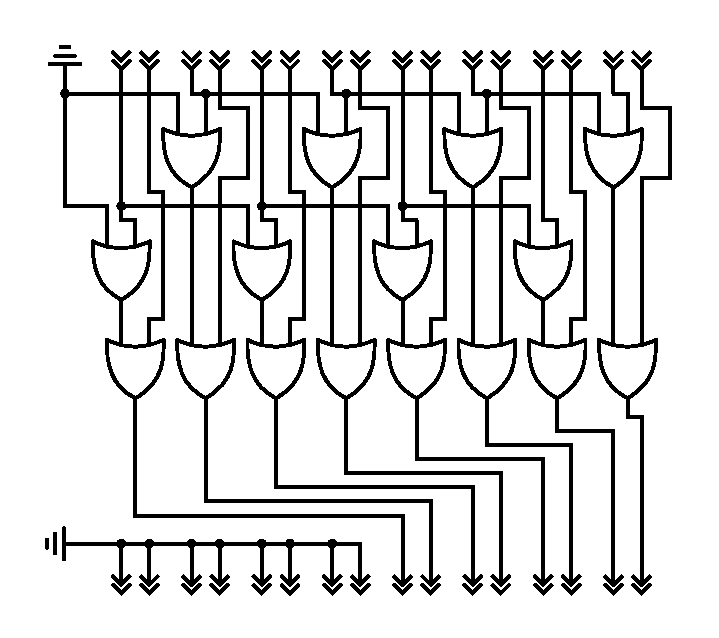
\includegraphics[width=0.75\linewidth]{figure/pdf/sqrt2Or.pdf} 
			\end{figure}

			Another algorithm for calculating square roots is the
			\emph{Shifting nth root algorithm}, also known as \emph{Dijkstras
			square root algorithm}, which calculates the square root one digit
			at a time. A \texttt{c} implementation of this algorithm is shown
			in figure \ref{sqrtc}. Initially, this algorithm does not seem like
			a good canditate for a high performance hardware implementation,
			but several important optimizations are possible when unrolling it
			combinatorially. Most of the additions can be reduced to bitwise
			logic operations already when computing it in software, as shown in
			figure \ref{sqrtcopt}. In a combinatorial hardware implementation,
			these bitwise operations can be removed entirely by simply moving
			wires around, yeilding a logic cost of 0. The only remaining
			operations is therefore the subtraction on line 6, and the
			conditional assignments of \texttt{num} and \texttt{res} on lines 9
			and 10. The cost of the subtraction can be significantly reduced
			because \texttt{res} approximates the result one bit every step,
			meaning most bits of \texttt{num} and \texttt{res} are zeroed at
			any given iteration. This means that on average, only 25\% of the
			subtraction logic is needed. This turned out to result in a design
			very similar to the PARSQRT implementation by \cite{Li}.

			\begin{table}
				\centering
				\caption{A \texttt{C} implementation of the shifting nth root 
					algorithm}
				\label{sqrtc}
				\begin{tabular}{c}
				\begin{lstlisting}
int isqrt(int num) {
    int res = 0;
    int bit = 1 << 30;

    while(bit != 0) {
        if(num >= res + bit) {
            num -= res + bit;
            res = (res >> 1) + bit;
        } else res >>= 1;
        bit >>= 2;
    }
    return res;
}
				\end{lstlisting}
				\end{tabular}
			\end{table}

			\begin{table}
				\centering
				\caption{A \texttt{C} implementation of the shifting nth root
					algorithm. This code example is slightly longer, but
					relatively expensive additions have been replaced by
					bitwise ors.}
				\label{sqrtcopt}
				\begin{tabular}{c}
				\begin{lstlisting}
int isqrt(int num) {
    int res = 0;
    int bit = 1 << 30;

    while(bit != 0) {
        int tmp = num - (res | bit);
        res >>= 1;
        if(tmp >= 0) {
            num = tmp;
            res |= bit;
        }
        bit >>= 2;
    }
    return res;
}
				\end{lstlisting}
				\end{tabular}
			\end{table}

